\chapter{Demonstração experimental das técnicas de aprendizado de máquina}\label{demonstracao-experimental-das-tecnicas-de-ml}
O experimento controlado apresenta os mecanismos de formação de arquétipos e de detecção de desvios sobre uma população de curvas sintéticas. A finalidade é examinar respostas distintas dos algoritmos em condições conhecidas; os resultados não correspondem a inspeções ou à prevalência de irregularidades na área de estudo.
\section{Demonstração controlada e limites de leitura dos gráficos}
Construíram-se 1.000 curvas diárias de 96 pontos, com resolução de 15 minutos. As famílias representaram consumo residencial noturno, comercial diurno, carga contínua e geração distribuída. Os perfis brutos conservaram amplitude. A normalização por dia evidenciou a distribuição relativa da energia, e os centroides do K-Means sintetizaram quatro famílias de morfologia. Na PCA, comparou-se a curva de entrada com a reconstruída. O erro euclidiano da Equação \eqref{residuo} localizou deformações mesmo quando a soma diária permaneceu semelhante.

\begin{equation}\label{residuo}
\varepsilon_i=\|\mathbf{x}_i-\widehat{\mathbf{x}}_i\|_2
\end{equation}
Os quatro grupos de curvas reuniram 443, 300, 156 e 101 observações, respectivamente. A Figura \ref{arquetipos} preserva os perfis individuais e a curva média de referência de cada grupo. O rótulo do arquétipo recupera a família geradora no exercício controlado. A forma de um perfil real exigiria interpretação em conjunto com a energia absoluta, a ocupação e o calendário.

\begin{figure}[htbp]\centering\caption{Arquétipos intradiários obtidos pelo K-Means nas 1.000 curvas sintéticas}\label{arquetipos}
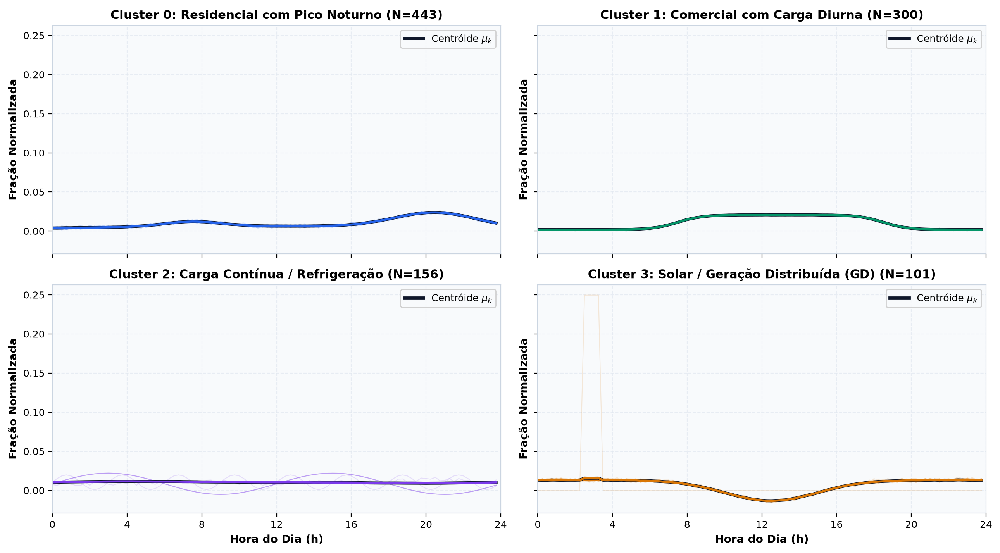
\includegraphics[width=0.96\textwidth,height=0.46\textheight,keepaspectratio]{figuras/arquetipos.pdf}
\par\small Fonte: elaboração própria com base na demonstração controlada.
\end{figure}
Na Figura \ref{pca}, as duas primeiras componentes explicaram 72,7\% e 17,1\% da variância, respectivamente. O erro de reconstrução mediu a parcela da curva que o subespaço retido não acomodou. Nos exemplos da Figura \ref{resid}, os resíduos foram 0,0075 e 0,0681. A diferença localizou uma deformação do perfil que a comparação de energia total poderia ocultar.

\begin{figure}[htbp]\centering\caption{Projeção, variância explicada e reconstrução na demonstração controlada}\label{pca}
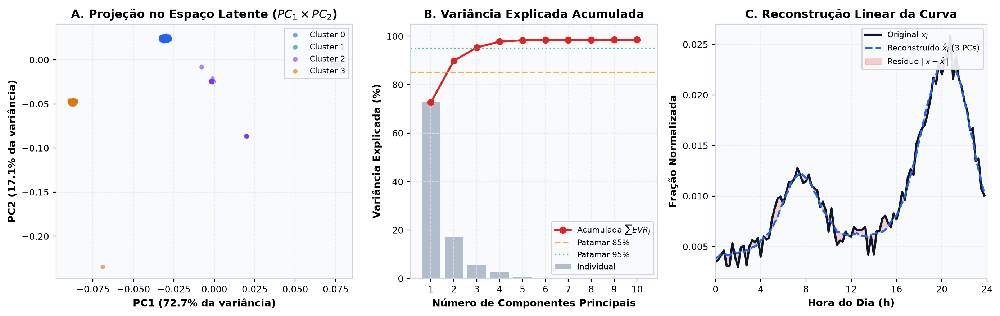
\includegraphics[width=0.96\textwidth,height=0.46\textheight,keepaspectratio]{figuras/pca.pdf}
\par\small Fonte: elaboração própria com base na demonstração controlada.
\end{figure}
\begin{figure}[htbp]\centering\caption{Erro de reconstrução de duas morfologias no subespaço da PCA}\label{resid}
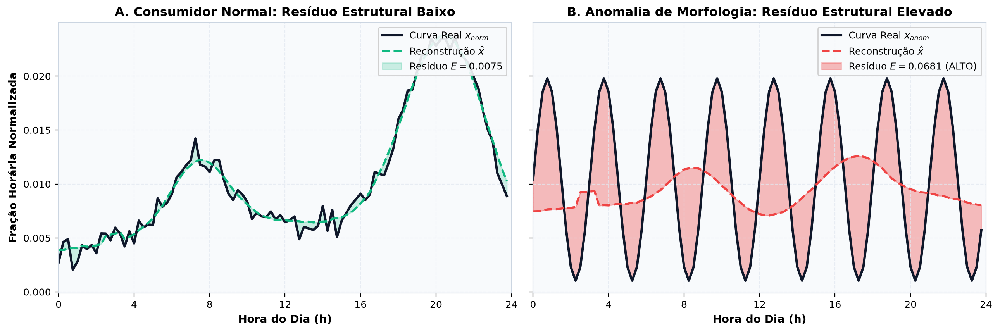
\includegraphics[width=0.96\textwidth,height=0.46\textheight,keepaspectratio]{figuras/resid.pdf}
\par\small Fonte: elaboração própria com base na demonstração controlada.
\end{figure}
Na demonstração de cobertura, atribuiu-se qualidade artificial aos perfis com semente 20261118. Oito casos receberam anomalias injetadas. A qualidade foi sorteada de uma distribuição beta com parâmetros (8, 2) nos demais casos e (7, 3) nos casos injetados. A Tabela \ref{sintetico} separa a permanência após o filtro da presença entre os primeiros 50 elegíveis. A associação entre menor qualidade e anomalia foi imposta pelo desenho sintético. A 70\%, apenas dois dos oito casos injetados permaneceram elegíveis e um integrou o Top-50. O resultado caracteriza a mecânica do filtro nesse ensaio, não sua sensibilidade para perdas não técnicas reais.

\begin{table}[htbp]\centering\small\caption{Retenção de oito anomalias injetadas na demonstração de cobertura}\label{sintetico}
\begin{tabular}{>{\raggedright\arraybackslash}p{\dimexpr 0.25\linewidth-2\tabcolsep\relax}>{\raggedright\arraybackslash}p{\dimexpr 0.25\linewidth-2\tabcolsep\relax}>{\raggedright\arraybackslash}p{\dimexpr 0.25\linewidth-2\tabcolsep\relax}>{\raggedright\arraybackslash}p{\dimexpr 0.25\linewidth-2\tabcolsep\relax}}\toprule
Cobertura mínima & Curvas elegíveis & Injetadas retidas & Injetadas no Top-50 \\ \midrule
40\% & 1.000 & 8 & 6 \\
50\% & 985 & 6 & 4 \\
60\% & 940 & 6 & 4 \\
70\% & 806 & 2 & 1 \\
80\% & 563 & 0 & 0 \\
90\% & 200 & 0 & 0 \\
\bottomrule\end{tabular}
\par\small Fonte: elaboração própria a partir dos dados e métodos do estudo.
\end{table}
O tempo medido na demonstração de 1.000 curvas foi de 441,40 ms para K-Means, 37,03 ms para PCA residual, 1.931,24 ms para IF, 14,29 ms para LOF e 1,39 ms para ECOD. O comitê composto consumiu 1.983,95 ms. O IF concentrou a maior parcela do tempo nesse ensaio. O número de vizinhos, o número de árvores, o tamanho da coorte e o paralelismo influenciam a comparação com outros ensaios.


\section{Interpretação dos detectores complementares}
O Isolation Forest separa observações por partições aleatórias, atribuindo maior raridade àquelas isoladas por caminhos curtos \autocite{liu2008}. O LOF compara a densidade local de uma observação à de seus vizinhos \autocite{breunig2000}; por isso, diferenças de escala e empates requerem controle. ECOD e COPOD empregam informações de caudas e distribuições empíricas \autocite{li2022ecod,li2020copod}; HBOS utiliza histogramas por atributo \autocite{goldstein2012hbos}, todos alinhados à formulação do ecossistema PyOD \autocite{zhao2019pyod}. O resíduo da PCA quantifica a distância entre o vetor e sua reconstrução no subespaço retido. Os detectores não são, a priori, independentes. A comparação de correlações e a retirada de componentes no ensaio OOT, descritas nos resultados, permitem avaliar a diferença entre suas ordenações sem pressupor ganho de precisão.


